\documentclass[12pt,a4paper]{article}
\usepackage[utf8]{inputenc}
\usepackage[T1]{fontenc}
\usepackage{amsmath, amssymb, amsthm}
\usepackage{geometry}
\usepackage{fancyhdr}
\usepackage{enumitem}
\usepackage{tikz}
\usepackage{animate}

\usepackage{blindtext}
\usepackage[hidelinks]{hyperref}
\usepackage{setspace}
\usepackage{float}
\usepackage{hyperref}
\usepackage{pdfpages}
\usepackage[hypcap=true]{caption} 
\hypersetup{hypertexnames=false} % Fixes duplicate identifier warnings
\usepackage{minted}

\definecolor{pastelred}{HTML}{FF7F7F}
\definecolor{pastelblue}{HTML}{9999FF}
\definecolor{pastelgreen}{HTML}{A8FFA8}

\setminted{
    breaklines=true,
    fontsize=\small,
    xleftmargin=0pt
}

\usepackage{comment}
\usetikzlibrary{calc,shapes.multipart,positioning,decorations.pathreplacing,arrows.meta}
\hypersetup{
    colorlinks=true,
    linkcolor=blue,
    filecolor=magenta,      
    urlcolor=cyan,
    pdfpagemode=FullScreen,
    }

\urlstyle{same}

\usepackage[most]{tcolorbox} % For the pretty terminal box
\newtcolorbox{terminalbox}{
    colback=gray!5!white,
    colframe=gray!40!white,
    fontupper=\small\ttfamily,
    sharp corners,
    boxrule=0.5pt,
    width=\linewidth,
    halign=left
}

\singlespacing{}

\setlength{\parindent}{0pt}
\setlength{\parskip}{0.5\baselineskip}

% Page Layout
\geometry{margin=1in}
\pagestyle{fancy}
\fancyhf{}
\lhead{CSE306 project 1 report}
\rhead{CSE306 EP}
\cfoot{\thepage}

\begin{document}

\title{\textbf{CSE306 project 1 report}}
\author{Cristian Verde}
\date{}
\maketitle

\section{Overview}

The objective of this project was to write a basic image renderer using ray tracing. The main C++ objects are a Scene and an Object which is extended by TriangleMesh and Sphere. The Scene is equipped with a camera position and a light position, together with a light intensity. Additionally, we have a lens diameter and a focal distance for depth of field, and a camera shutter time for motion blur (which are all optional but provide nice images).

Additionally, each Object can have a velocity vector (for motion blur), and a \texttt{is\_light} boolean variable to create non-point light sources (a spherical light source, for instance).

\section{Results}

The following images (and gif) were generated on my local machine running an Intel i7-13700H with 14 cores (6 fast with 2 threads each and 8 with only 1 thread, totalling 20 threads). The times are collected using the standard \texttt{time} program and each one is ran only once because I did not observe significant deviations. The compilation flags relevant for performance were \texttt{-O3 -fopenmp -ffast-math}.

For ease, I will time everything with 64 samples (apart from lab 1), a 512x512 picture and 5 light bounces (if not specified otherwise).

\subsection{Lab 1}

\begin{figure}[H]
	\centering
	\begin{minipage}[c]{0.48\textwidth}
		\centering
		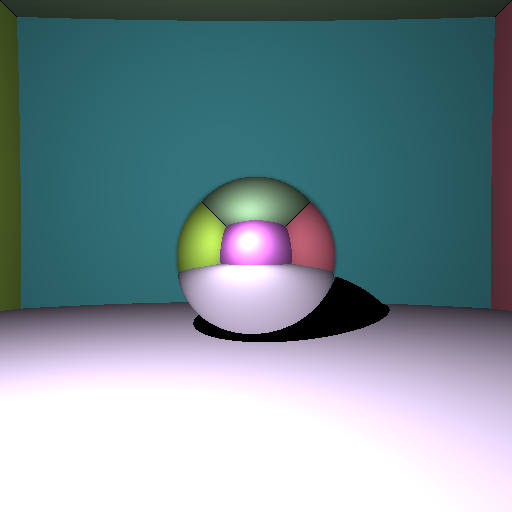
\includegraphics[width=\textwidth]{../lab1.png}
		\caption{Result at the end of lab 1.}
	\end{minipage}
	\hfill
	\begin{minipage}[c]{0.45\textwidth}
		\raggedright
		\textbf{Execution metrics:}
		\vspace{0.5em}
		\begin{terminalbox}
			real    0m0.027s\\
			user    0m0.132s\\
			sys     0m0.003s
		\end{terminalbox}
	\end{minipage}
\end{figure}

There is not much to say about this one. We send a ray in each direction (which is actually the ray that enters the camera, but ``tracing the steps back'' is what helps us see where the ray came from). We see what object (if any) is hit first, and if there is another object between this object and the light source, we have a shadow. The edges are ragged because there is no sampling yet, so each pixel ``belongs'' to at most one object (there is no blending). The generation time is also really fast because there is no sampling.

\subsection{Lab 2}

\begin{figure}[H]
	\centering
	\begin{minipage}[c]{0.48\textwidth}
		\centering
		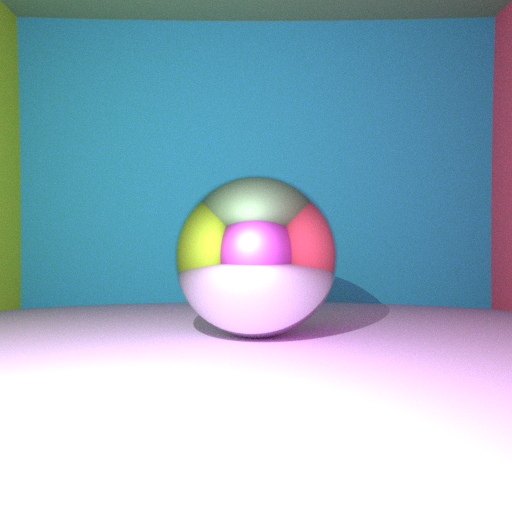
\includegraphics[width=\textwidth]{../lab2.png}
		\caption{Result at the end of lab 2.}
	\end{minipage}
	\hfill
	\begin{minipage}[c]{0.45\textwidth}
		\raggedright
		\textbf{Execution metrics:}
		\vspace{0.5em}
		\begin{terminalbox}
			real    0m3.574s\\
			user    1m9.224s\\
			sys     0m0.030s
		\end{terminalbox}
	\end{minipage}
\end{figure}

\begin{figure}[H]
	\centering
	\begin{minipage}[c]{0.48\textwidth}
		\centering
		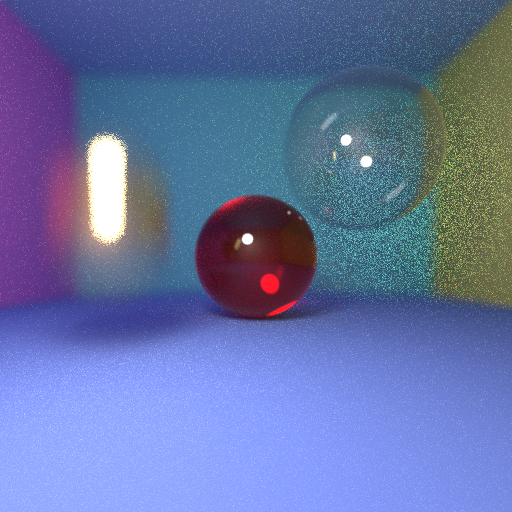
\includegraphics[width=\textwidth]{lab2_cooler_remake.png}
		\caption{Lab 2 made cooler (extra work). Also, 500 samples and 10 light bounces.}
	\end{minipage}
	\hfill
	\begin{minipage}[c]{0.45\textwidth}
		\raggedright
		\textbf{Execution metrics:}
		\vspace{0.5em}
		\begin{terminalbox}
			real    2m44.396s\\
			user    54m13.604s\\
			sys     0m1.163s
		\end{terminalbox}
	\end{minipage}
\end{figure}

In this lab, we added sampling for anti-aliasing. This means we now shoot 64 rays in each direction, but with a slight deviation, and we average all the colors we get, to even out the edges (this basically blends the colors at the edges). We also add an indirect light component for ``softer'' shadows (otherwise they would be pitch black) by shooting a ray from the collision point.

The result is about 500 times slower than before, due to 64*5 more operations, and some cache misses due to our non-\texttt{thread\_local} random number generation.

Disclaimer, everything in the second photo was added outside of the lab. Transparency, motion blur, depth of field, and the ``inverse normal'' trick to make a glass sphere. The time is actually measured without Russian roulette (therefore I send two separate rays in case of refraction, and having 2 transparent spheres, it takes a lot of time$\ldots$). The light source itself is a sphere, which is why the shadows (especially for the transparent sphere) are so grainy.

\subsection{Lab 3}

\begin{figure}[H]
	\centering
	\begin{minipage}[c]{0.48\textwidth}
		\centering
		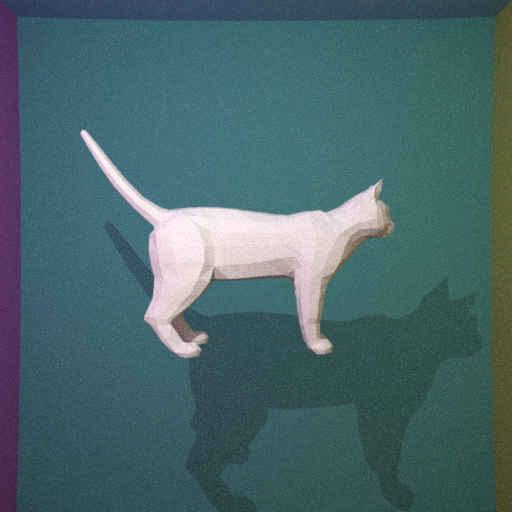
\includegraphics[width=\textwidth]{lab3_remake.png}
		\caption{Result at the end of lab 3. Cat with 3954 triangles.}
	\end{minipage}
	\hfill
	\begin{minipage}[c]{0.45\textwidth}
		\raggedright
		\textbf{Execution metrics:}
		\vspace{0.5em}
		\begin{terminalbox}
			real    1m54.344s\\
			user    37m27.170s\\
			sys     0m0.888s
		\end{terminalbox}
	\end{minipage}
\end{figure}

This lab adds triangle meshes. We can now import a .obj file, and we just had to implement the intersection function following some formulas. The running time is pretty bad, but currently we are traversing all 3954 triangles for every ray which hits the bounding box of our object.

\subsection{Lab 4}

\begin{figure}[H]
	\centering
	\begin{minipage}[c]{0.48\textwidth}
		\centering
		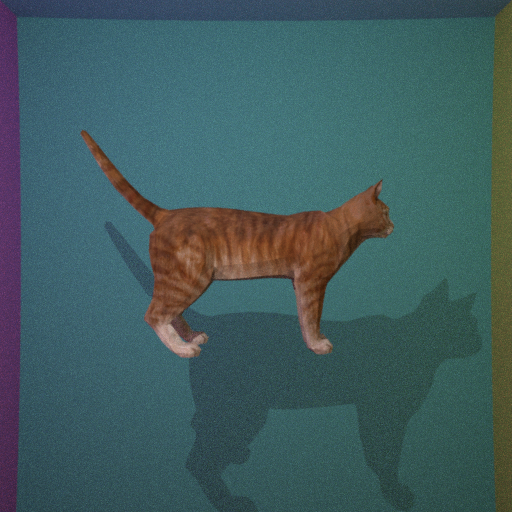
\includegraphics[width=\textwidth]{lab4_remake.png}
		\caption{BVH reduced running time considerably, and added textures.}
	\end{minipage}
	\hfill
	\begin{minipage}[c]{0.45\textwidth}
		\raggedright
		\textbf{Execution metrics:}
		\vspace{0.5em}
		\begin{terminalbox}
			real    0m3.971s\\
			user    1m16.903s\\
			sys     0m0.053s
		\end{terminalbox}
	\end{minipage}
\end{figure}

Because Bounded Volume Hierarchy (BVH) takes us from linear time when a ray hits the bounding box to roughly-logarithmic by segmenting the cats in smaller bounding boxes, we observe a massive speed-up of about 28x.

\subsection{Miscellaneous stuff}

\begin{figure}[H]
	\centering
	\href{https://imgur.com/a/mKup0pa}{
		
\includegraphics[width=0.6\textwidth]{../cat_gif_new/frame_000.png}
	}
	\caption{144-frame animation of Dingus using ffmpeg, available \textbf{\href{https://imgur.com/a/mKup0pa}{here}}.}
\end{figure}

\subsection{Potential improvements}

It is far from optimal (for example, each \texttt{std::default\_random\_engine} could be \newline \texttt{thread\_local}, which would remove the cache misses and incur a considerable speed-up of about 30\% post-BVH, when this becomes a bottleneck). Moreover, it is one huge 1100-line file which is ugly. Also, for transparency, the current code does Russian roulette, which is faster than shooting two different rays but I acknowledge it is worse with how many samples we are working with.

Upon further testing, by improving the math inside the TriangleMesh intersection, I could improve the efficiency by 2x (before BVH). However, I will not further modify the code.

\end{document}
